\section{Design}
In this section we have designed the system and created class diagrams for the various parts of the system.

\subsection{Server-side}
The diagram shown on \ref{fig:serversidestructure} describes the overall structure of the server-side of the system. The server-side consists of both the Web-API and the control panel. These has been combined since they both interact with the same database and both has the same model. 

\begin{figure}[H]
    \centering
    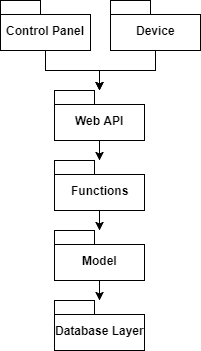
\includegraphics{Figures/serverSide.png}
    \caption{The structure of the server-side part of the system}
    \label{fig:serversidestructure}
\end{figure}

The function-layer is split into two parts, one for the control-panel and one for the API. This is done to isolate the functionality, such that each component only has access to their needed functionality. The shared model layer is described on \ref{fig:serversidemodel}.

\begin{figure}[H]
    \centering 
    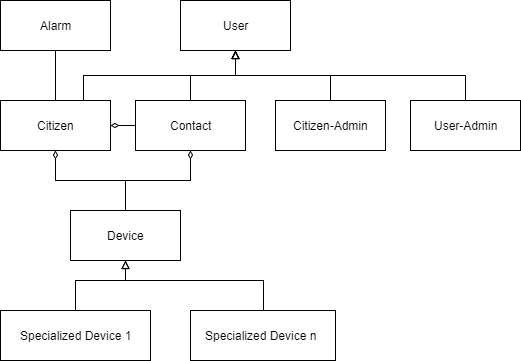
\includegraphics[width=0.9\textwidth] {Figures/serverSidemodel.png}
    \caption{The serverside model}
    \label{fig:serversidemodel}
\end{figure}
This class-diagram describes the model-layer, and the relations between the different parts of the model-layer.

\subsection{Web-API}

\subsubsection{REST}

\subsubsection{WSDL}

\subsubsection{SOAP}


\subsection{Control panel}
The diagram shown on \ref{fig:controlpanel} describes the different views in the control panel. The login view is the view shown, when a user must login to the control panel.\\
The admin view, is the view shown to users with administration rights. The view will make the admin able to add new users to the system from the view.\\
The citizen view is for users with citizen-admin rights. The view will show the information on all the citizen the citizen-admin is administrating.

\begin{figure}[H]
    \centering
    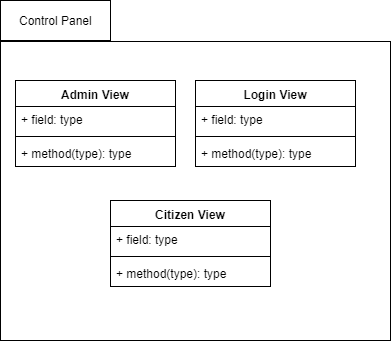
\includegraphics[width=0.7\textwidth]{Figures/ControlPanel.png}
    \caption{The different views included in the control-panel}
    \label{fig:controlpanel}
\end{figure}

\subsection{Smartphone app}

\subsection{Personal assistant}